\chapter{Testování softwaru}
%SMAZAT!!
%Testování aplikací je nedílnou součástí jejich vývoje a~v~dnešní době se tomuto oddílu tvorby aplikací věnuje čím dál více pozornosti. Dá se rozdělit do různých skupin, např. podle toho, kdy se testování provádí, jakým způsobem se provádí, jak se k~testované aplikaci přistupuje, či jaká část aplikace se podrobuje testům.

%Jednou z~důležitých součástí je testování grafického uživatelského rozhraní. Zde se testeři soustředí na to, zda daná aplikace vypadá tak, jak to požadují vývojáři a~návrh, a~zda grafické prvky správně fungují. Dále se zaměřuje na to, zda je aplikace přívětivá k~uživateli a~práce s~ní není příliš komplikovaná.

%Při testování grafického uživatelského rozhraní se může spousta testů mnohokrát opakovat, a~proto je snaha tyto testy nějak automatizovat. K~tomu se může využít některý z~nástrojů k~tomu určený. Cílem této práce je seznámit se s~některými z~těchto nástrojů, jeden z~nich vybrat a~pomocí něj vytvořit sadu ukázkových testů svou filosofií zapadajících do předmětu KIV/OKS.

Na začátek je potřeba vysvětlit některé pojmy z~oblasti testování. Budeme vycházet hlavně z~\citep{RizeniKvalitySW}.

	\section{Požadavky}
	Požadavky zachycují přání zákazníka na funkcionalitu softwaru. Dělí se na dvě skupiny:
		\begin{itemize}
			\item Funkční -- popisují funkčnost služby vykonávané systémem, tedy co má vykonávat. Patří sem např.:
				\begin{itemize}
					\item Uživatel bude moci vytvořit záznam pro nového zákazníka.
					\item Systém automaticky odhlásí uživatele po 3 minutách nečinnosti.
				\end{itemize}
			\item Mimofunkční -- popisují určité vlastnosti systému, či omezující podmínky. V podstatě říkají, jaký by systém měl být. Sem patří např.:
				\begin{itemize}
					\item Modul "Správa klientů" bude dostupný pouze uživatelům s~rolí správce.
					\item Systém bude použitelný při zátěži 1000 uživatelů.
				\end{itemize}
		\end{itemize}
	
	Je vhodné, aby se testeři zabývali i~požadavky, neboť mohou již v~rané fázi vývoje zachytit ty chybně formulované (nekonzistentní, neproveditelné, nekompletní, netestovatelné, nejednoznačné, více požadavků zapsaných jako jeden apod.).
	
	\section{Specifikace požadavků na software}
	Funkční i~mimofunkční požadavky zákazníka, jejich analýza a~dokumentace a~všeobecný popis systému se zapisuje do dokumentu nazvaného specifikace požadavků na software. Na základě tohoto dokumentu probíhají následující fáze vývoje, proto je jeho správnost velmi podstatná.
	
	K~tomuto dokumentu se poté vztahuje i~testování, konkrétně funkční testování, které kontroluje, zda software vyhovuje a~splňuje požadavky zákazníka.
	
	\section{Kvalita softwaru}
	Kvalita softwaru je velmi obtížně definovatelný pojem. Pro její definici vzniklo několik norem. Ty jsou dnes zastaralé či nekonzistentní, proto jsou nahrazovány jednotným systémem norem ISO/IEC 25000-25099 v~rámci projektu SQuaRe (Software Quality Requirements and Evaluation).
	
	Např. norma ISO/IEC 25010 říká, že kvalita softwaru je míra, do jaké softwarový produkt splňuje stanovené a~implicitní potřeby, je-li používán za stanovených podmínek.
	
		\subsection{FURPS}
		Dnes nejčastějším modelem kvality softwaru je tzv. FURPS, který vytvořila společnost Hewlett-Packard. Ten kvalitu popisuje pomocí těchto pěti charakteristik:
			\begin{itemize}
				\item Funkčnost -- soubor požadované funkcionality, schopností a~bezpečnostních aspektů systému.
				\item Použitelnost -- snadnost použití, konzistence, estetika, dokumentace apod.
				\item Spolehlivost -- četnost a~závažnost selhání, doba bezporuchového běhu, správnost výstupů, zotavení atd.
				\item Výkonnost -- odezva systému, výkon za různých podmínek, požadavky na systémové prostředí.
				\item Rozšiřitelnost/podporovatelnost -- škálovatelnost, udržovatelnost, testovatelnost, snadnost konfigurace.
			\end{itemize}
		Většinou se setkáme s~modelem FURPS+, který navíc přidává kategorie jako omezení návrhu, požadavky na implementaci, požadavky na rozhraní a~požadavky na fyzické vlastnosti.
			
	\section{Chyba, defekt, selhání}
	Během vývoje softwaru se do dokumentů či zdrojových kódů dostávají defekty, způsobující chyby a~selhání. Tyto pojmy je velmi důležité rozlišovat. V~následujících odstavcích bude jejich význam vysvětlen.
	
	Selhání nastává v~případě, že jeden nebo více výstupních stavů aplikace se odlišuje od stavu správného (nesplňuje specifikaci, případně specifikace nebyla kompletní nebo jednoznačná).
	
	Právě toto odchýlení od očekávaného stavu se nazývá chybou. Původ chyby se nazývá defekt a~označuje se tak vada v~kódu či datech. Nejčastěji jej způsobí programátor chybou v~kódu, špatným návrhem, nedostatečně či nesprávně pochopenou specifikací, nebo záměrnou sabotáží.
	
	Jednotlivé pojmy na sebe tedy navazují následovně (viz obrázek \ref{Bug}): defekt (aktivace) $\to$ chyba (šíření) $\to$ selhání (příčina) $\to$ defekt\dots
	\begin{figure}[ht!]
		\centering
		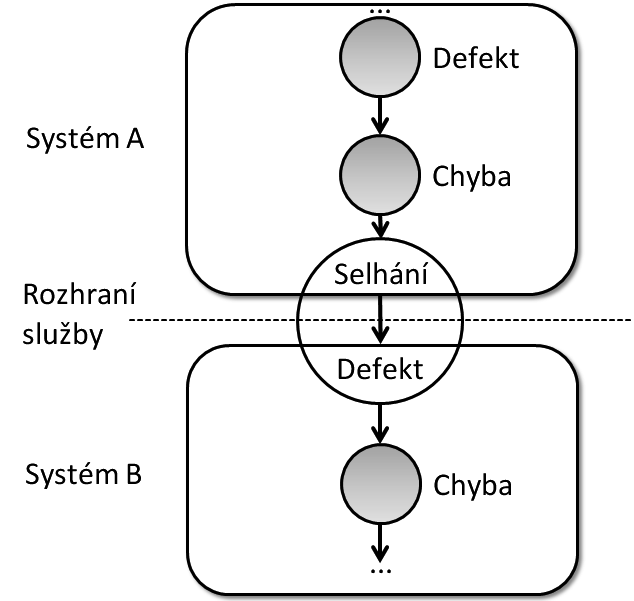
\includegraphics[width=8cm]{img/Bug.png}
		\caption{Šíření chyby mezi systémy. Selhání systému A je pro příjemce jeho služby (systém B) externím defektem, který může vést k~chybě a~ta poté opět  k~selhání. Zdroj \citep{RizeniKvalitySW}}
		\label{Bug}
	\end{figure}